\setlength{\headheight}{15pt}
\chapter{Multilingual Topic Classification in X: Dataset and Analysis}
\label{ch:x-topic}

% added for thesis
In the previous Chapter, \Autoref{ch:tweet-topic}, we introduced the task of tweet topic classification, presented an English-language dataset, and evaluated several transformer-based models. In this Chapter, we expand the scope of the task to include multiple languages. We introduce {\XTOPIC}, a multilingual dataset featuring content in four distinct languages (English, Spanish, Japanese, and Greek), crafted for the purpose of tweet topic classification. The dataset utilises the same taxonomy as {\TweetTopic}, ensuring direct comparability across languages and enabling consistent evaluation in both monolingual and multilingual settings, making it a valuable resource for scientists and professionals working on cross-linguistic analysis, the development of robust multilingual models, and computational scientists studying online dialogue. By providing parallel resources across multiple languages, {\XTOPIC} addresses the lack of high-quality, in-domain multilingual datasets for supervised topic classification in social media. We use {\XTOPIC} to conduct a comprehensive cross-linguistic and multilingual evaluation, comparing the performance of current general-purpose and domain-specific \acp{LM} and analysing the challenges that arise in this setting.

This chapter reproduces verbatim our paper \textit{Multilingual Topic Classification in X: Dataset and
Analysis}, published in the Proceedings of the Conference on Empirical Methods in
Natural Language Processing, 2024 (\Autoref{ch:intro:publications}, \Autoref{publication:2}), with only minor modifications to presentation. It corresponds directly to the contributions outlined in \Autoref{ch:intro:contributions}, specifically \Autoref{contribution:1}, \textit{New Datasets for Topic Classification on Twitter}.


\selectlanguage{english}
\section{Introduction}
Social platforms such as \textit{X} , Snapchat and Instagram provide an environment for content creation and information sharing among people and organisations. In particular, people use these platforms to express their sentiments, share their opinions on multiple topics, and discuss and influence each other \cite{barbieri-etal-2014-modelling,hu2021revealing,ansari2020analysis}. In this scenario, these platforms are rich sources for informal short text, as they include content about recent events, shared by a heterogeneous group of users. The vast amount of content shared on social media, however, make it impossible to analyse and digest it without automatic tools.

Unsupervised approaches such as \ac{LDA} \cite{lda} and topic modelling variations \cite{steyvers2007probabilistic}, or more recently, BERTopic \cite{bertopic}, are common approaches to deal with this issue.
However, these methods are usually built as an ad-hoc analysis, with the derived topics not being easily interpretable or comparable among different analyses. On the other hand, when looking at supervising approaches, existing resources mainly focus on the news articles domain, e.g., BBC News \cite{greene2006practical}, Reuter \cite{lewis2004rcv1}, 20News \cite{lang1995newsweeder}, and WMT News Crawl \cite{lazaridou2021mind} with few exceptions like scientific (arXiv) \cite{lazaridou2021mind} and medical (Ohsumed) \cite{hersh1994ohsumed} domains. 


This Chapter focuses on expanding the resources available for multilingual tweet classification. 
We leverage an initial topic taxonomy of 19 topics, first proposed in \newcite{antypas2022twitter}, and introduce the new {\XTOPIC} dataset that includes tweets from four different languages: English, Spanish, Japanese and Greek. Our dataset is focused on \textit{X} data and aims to address the lack of labelled multilingual social media data, as well as to encourage the creation of new methods for multilingual topic classification. 

By leveraging {\XTOPIC} as a benchmark, we explore multiple model architectures and sizes for multilingual tweet topic classification: 
(1) zero-shot, (2) few-shot, (3) monolingual, (4) cross-lingual and (5) multilingual. Our analysis highlights the challenging nature of the task and reveals interesting patterns in relation to the use of \acp{LLM} and supervised approaches for the topic classification task in social media, especially in relation to the type of data considered for training. 

The {\XTOPIC} dataset, as well as the topic classification models built upon it, are made openly available. {\XTOPIC} is available at \url{https://huggingface.co/datasets/cardiffnlp/tweet_topic_multilingual}. Table \ref{tab:examples} shows some sample instances of {\XTOPIC} for each language. Finally, the best multilingual models of \textit{base} and \textit{large} sizes are available at \url{https://huggingface.co/cardiffnlp/twitter-xlm-roberta-base-topic-multilingual} and \url{https://huggingface.co/cardiffnlp/twitter-xlm-roberta-large-topic-multilingual}, respectively.



\begin{table}[!ht]
\centering
\scalebox{0.7}{
\begin{tabular}{l|l}
\multicolumn{1}{c|}{\textbf{Tweet}} & \multicolumn{1}{c}{\textbf{Topics}} \\
\begin{tabular}[c]{@{}l@{}}\textbf{en}: I don’t think I really want to go to  Coachella  unless Taylor Swift is headlining\end{tabular} & Celebrity \& Pop Culture, Music \\ \hline
\begin{tabular}[c]{@{}l@{}}\textbf{es}: quiero una date en un museo\\ \\ \textbf{translation}: I want a date in a museum\end{tabular} & \textit{\begin{tabular}[c]{@{}l@{}}Relationships, Arts \& Culture,\\ Diaries \& Daily Life\end{tabular}} \\ \hline
\begin{CJK*}{UTF8}{min}\begin{tabular}[c]{@{}l@{}}\textbf{ja}: 久々になーーんもしないでいい日が二日もあるのでゆっくり富平井絆果と\\向き合うよ\\ \\ \textbf{translation}: It's been a long time since I've had two  days where I don't have to do anything, \\ so I'm going to take my time and face Kizuna Fuhirai.\end{tabular}\end{CJK*} & \textit{Diaries \& Daily Life, Gaming} \\ \hline
\begin{tabular}[c]{@{}l@{}}\textbf{gr}:\selectlanguage{greek} Μπα σε καλό σου μωρή Ανθουλα μας κοψοχολιασες πάλι \#σασμός\\ \\ \textbf{translation}: Oh my goodness, Anthula, you've cracked us up again  \#sasmos\end{tabular} & Film, TV \& Video
\end{tabular}
}
\caption{Example of tweets present in each language subset of \XTOPIC.}\label{tab:examples}
\end{table}

\section{Related Work}

The task of classifying topics in social media content has garnered significant attention from the research community in recent years \cite{schlichtkrull2023intended,10.1145/3161603,chua2016linguistic}. Social media platforms like \textit{X} have become hubs for the exchange of information, opinions, and sentiments, making the development of effective classification methods imperative. 

\paragraph{Unsupervised Approaches.}
Due to the lack of labelled data and the dynamic nature of social media platforms, unsupervised methods have been widely used for topic modelling and classification on the content shared. Several variations of \ac{LDA} have been introduced that try to address the challenges that arise when working with the often messy and unstructured world of social media. Such solutions, \cite{zhao2011comparing,rosen2004author,steinskog-etal-2017-twitter} often try to  combine author information with the text shared.
Other approaches use unsupervised clustering algorithms, such as k-means or hierarchical clustering, to group similar social media content based on their topic similarity \cite{10.1007/978-3-319-67256-4_30}. These methods are particularly useful when the underlying topics are not predefined and need to be inferred from the data. However, a drawback of these unsupervised approaches is that the derived topics may not always be easily interpretable or comparable across corpora.


\paragraph{Multilingual resources in social media.}
Supervised methods for topic classification in social media content involve \ac{ML} learning models on labelled data. While supervised approaches have demonstrated robust performance on social media tasks \cite{huang2013sentiment,camacho2022tweetnlp}, there is a notable scarcity of labelled data for social media content, particularly in languages other than English \cite{selvaperumal2014short}; while a lot of the available datasets offer a limited taxonomy of topics \cite{vadivukarassi2019comparison}. 
Multilingual and cross-lingual topic classification in social media is therefore a limited explored area. It involves dealing with content in multiple languages, addressing language-specific nuances, and ensuring effective classification. Few resources and models are designed to handle multilingual topic classification. Existing datasets e.g. in Portuguese \cite{daouadi2021optimizing}, Spanish \cite{imran2016twitter}, Urdu \cite{kausar2021hashcat} and others \cite{chowdhury2020cross}, often suffer from weak labelling or a limited taxonomy of topics, or they are created to solve specific problems e.g. sentiment analysis \cite{muhammad2023semeval} and hate speech \cite{ousidhoum-etal-2019-multilingual}. %politics, natural disasters
This presents a gap in the field as many social media platforms have a global user base. Our work addresses this gap by introducing the {\XTOPIC} dataset, which includes tweets in four different languages (English, Spanish, Japanese, and Greek), thereby expanding resources for multilingual topic classification in social media. 


\section{\XTOPIC, a Multilingual Tweet Topic Classification Benchmark}

In this section, we describe our methodology to construct, a multilingual tweet topic classification benchmark. First, we describe the original English-based \TweetTopic dataset, which we take as inspiration to construct a fully multilingual dataset.

{\TweetTopic} \cite{antypas2022twitter} is an English Twitter topic classification dataset consisting of a total of 11,267 English tweets assigned one or more classes from a predefined list of 19 topics such as "News \& Social Concern", "Sports", and "Fashion \& Style". The taxonomy of topics was decided by a team of social media experts and aims to cover the majority of content being shared in social media platforms. The tweets were distributed over time, from September 2019 to October 2021 and were extracted using keywords of trending topics in each week during the period. Each entry was labelled by five different annotators, and the topic was assigned if there was an agreement of at least two annotators. 


In our work, we leverage the taxonomy originally presented in {\TweetTopic} as a foundation for collecting a new set of recent tweets, leading to the introduction of {\XTOPIC}. {\XTOPIC} is mainly distinguished by its inclusion of entries in four diverse languages: Spanish, Greek, Japanese, and English. 

\subsection{Language Selection and Tweet Collection}

The selection of languages was made by taking into account their popularity and practicality. {\XTOPIC} is a resource that helps to the analysis of frequently used languages in \textit{X} (English, Spanish, Japanese) as well as a less frequently studied one (Greek). This linguistic diversity also provides a unique opportunity for comparative analysis between linguistically distant groups, such as Japanese and Greek. Moreover, our choice of the September 2021 to August 2022 timeframe continues the timeline of previous work and facilitates engaging in temporal analyses.


For the collection of the dataset, we follow a similar approach to that of the original {\TweetTopic}. Initially, the Twitter API was utilised to collect 50 tweets every two hours for each language. However, in contrast to {\TweetTopic}, we do not use any keyword filtering in our queries. In this way, we acquire a diverse set of tweets, approximately 220,000 tweets for each language, which is closer to the real distribution of content shared in \textit{X}. 



\subsection{Preprocessing}
\label{sec:preprocessing}

Following the collection of the raw tweets we apply several preprocessing steps. First, we remove potentially remaining tweets in other languages by using a fastText-based language identifier \cite{bojanowski2017enriching} on top of the Twitter pre-defined language identifier. Then, we remove tweets that are not in our target period, tweets containing incomplete sentences (too short or end in the middle of the sentence), or abusing words by applying some simple rule-based heuristics. We also apply a \textit{near-duplication} filter to drop duplicated tweets. This process begins by normalising each tweet (i.e. remove irrelevant substrings and lemmatisation), and then retaining unique tweets only in terms of the normalised form. To ensure the quality of the tweets' content we remove entries that contain URLs, and those where multiple (more than four) emojis or mentions are present.\footnote{Detailed number of tweets dropped in each preprocessing step can be found in Table \ref{tab:preprocessing_steps}, Appendix \ref{appendix:Xtopic-dataset}.} Finally, we sample 1,000 tweets from the remaining set of tweets after preprocessing for each language. The sampling is weighted based on the retweet count of each entry as well as the follower count of the user posting the tweet. This weighting is applied with the assumption that a higher quality content is usually more popular. As a final preprocessing step we mask all mentions of non-verified users with \{USER\} to ensure the privacy of users. 



\subsection{Annotation}
\label{sec:annotation}
The annotation process closely mirrored the procedure established in {\TweetTopic}. Specifically, each entry of the dataset was annotated by five coders, where each coder had to select one or more labels from a selection of 19 topics in total. A topic was assigned to a tweet only if at least two annotators were in agreement about it. Following previous work on multi-label classification \cite{mohammad2018semeval}, we refrained from utilising a majority rule in order to create a more realistic and challenging dataset.



The coders who worked on this task were selected and filtered through the \textit{Prolific.co} platform based on their fluency in the corresponding target language. 

The actual annotation was performed through an interface created with qualtrics\textsuperscript{XM}.\footnote{The annotation guidelines for each language can be found in Appendix \ref{appendix:XTopic-guidelines}.} We did not utilise Amazon Mechanical Turk (AMT) due to both the lack of non-English annotators in AMT, as well as, due to the better quality of annotators present in \textit{Prolific.co}. Finally, we ensured the quality of the annotations as our research team includes native speakers in all the non-English languages, who monitored the whole annotation process for each language.

\begin{figure}
    \centering
    \scalebox{0.75}{
    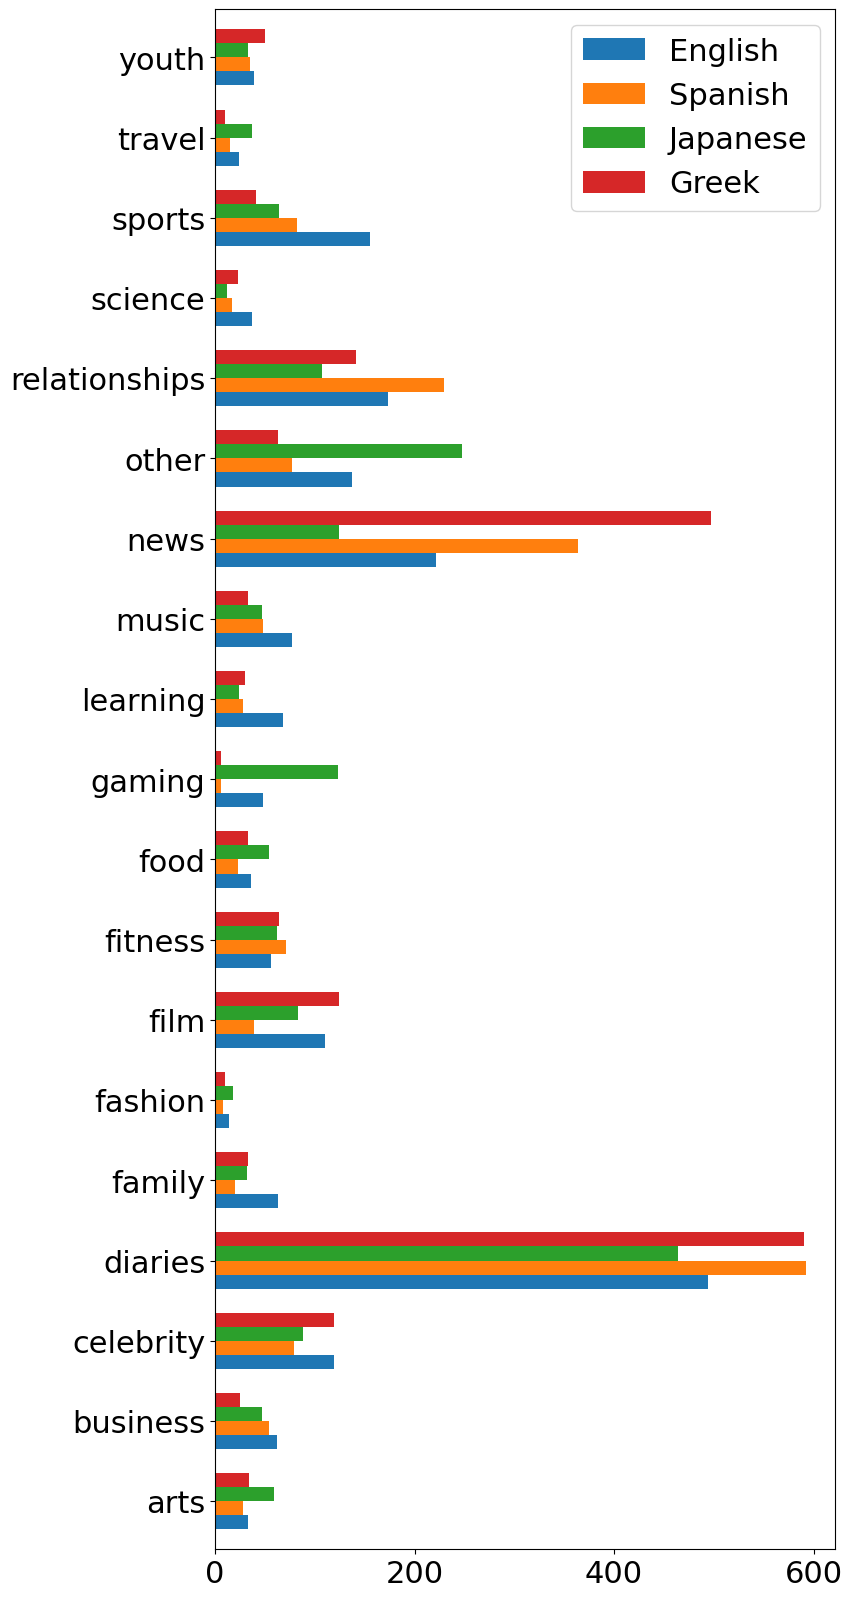
\includegraphics[width=\textwidth]{../figures/x-topic/topic_distribution.png}}
    \caption{Number of tweets per topic and language.}
    \label{fig:topic-distribution}
\end{figure}

 %Inter-Annotator Agreement (\textit{IRA})
To assess the quality of our annotation process, we report the following three annotation agreement metrics: (1) Krippendorff's Alpha (\textit{Alpha}) \cite{krippendorff2011computing}, (2) Percent Agreement  (\textit{PA}), ratio of number of agreements to the total number of annotations, and (3) Agreement between each pair of coders on at least one label (\textit{Overlap}). When comparing our results with those achieved in the {\TweetTopic} annotation, as presented in Table \ref{tab:annotators-agreement}, we can observe an overall smaller concordance 
 among coders. The highest \textit{Alpha} score observed was 0.26 in the Greek dataset, in contrast to {\TweetTopic}'s 0.34. Nevertheless, the agreement metrics remain on par with similar multi-label annotation tasks such as the datasets \textit{Affect in Tweets}, with a Fleiss' Kappa score of 0.26, \cite{mohammad2018semeval} and \textit{GoEmotions} \cite{demszky-etal-2020-goemotions}, with an \textit{Alpha} score of 0.24, noting that a random annotation process would yield an \textit{Alpha} score of 0.


\begin{table}[ht]
\centering
\scalebox{1}{
\begin{tabular}{l|c|c|c|c}
                    & \textbf{Alpha} & \textbf{ PA } & \textbf{Overlap}  & \textbf{AVG Topics}\\ \hline%(at least 1 class)
\textbf{English}    & 0.23                                                                   & 0.87     & 0.60  & 2.0 \\
\textbf{Spanish}    & 0.23                                                                   & 0.89     & 0.63  & 1.8\\
\textbf{Japanese}   & 0.21                                                                   & 0.87     & 0.48  & 1.7\\
\textbf{Greek}      & 0.26                                                                   & 0.89     & 0.74  & 1.9 \\ \hline\hline
\textbf{TweetTopic} & 0.34                                                                   & 0.90     & 0.70  & 1.6      
\end{tabular}}

\caption{Annotator agreement in each language subset of {\XTOPIC} and {\TweetTopic}, as well as the average number of topics (\textit{AVG Topics}) assigned to each tweet.}
\label{tab:annotators-agreement}
\end{table}




\subsection{Descriptive Analysis}

{\XTOPIC} encompasses a total of 361 distinct topic combinations within its 4,000 tweets, showcasing its diversity in themes and coverage. In Table \ref{tab:examples}, we present illustrative entries from our dataset for each language, displaying various topics. Notably, each tweet, on average, is associated with 1.8 topics, with none of the entries assigned more than 5 topics.


\paragraph{Topic overlap.} Upon examining the overlap between topics across all languages, as depicted in Figure \ref{fig:overlap}, Appendix \ref{appendix:Xtopic-dataset}, we observe interesting patterns. For instance, the \textit{diaries\_\&\_daily\_life (diaries)}  topic frequently co-occurs with other topics, such as \textit{family} (79\%) and \textit{relationships} (76\%). Furthermore, there is a substantial overlap between topics %that align with expectations. a
that we expected to be closely related in online discussions.
For instance, \textit{music} and \textit{celebrities\_\&\_pop\_culture} exhibit a 45\% overlap, while \textit{youth\_\&\_student\_life (youth)} and \textit{learning\_\&\_educational (learning)} demonstrate a 25\% overlap.

\paragraph{Topic distribution.} As seen in Figure \ref{fig:topic-distribution}\footnote{A map of topic name abbreviations is provided in Appendix \ref{appendix:XTopic-topic_abbreviations}.}, \textit{diaries\_\&\_daily\_life} is the majority class across all four language subsets with 494, 592, 464, and 590 tweets present in English, Spanish, Japanese, and Greek respectively. When looking at less popular topics, differences between languages start becoming apparent with \textit{news\_\&\_social\_concern} being the second most popular topic for English, Spanish, and Greek (221, 364, and 497 tweets respectively), and \textit{other\_hobbies} being the second most popular topic in Japanese (248 tweets). This is in contrast to the {\TweetTopic} dataset which also exhibits an imbalanced distribution but to a lesser degree. This difference can be explained by the fact that in {\XTOPIC} we randomly extract tweets from \textit{X}, aiming to replicate a realistic distribution, rather than utilising trending keywords. These variations in the topic distributions among the four languages, along with differences in the average post length (average number of characters: en: 149.02, es: 128.93, gr: 144.71, ja: 48.58) and the usage of emojis (average number of emojis: en: 0.43, es: 0.42, gr: 0.25, ja: 0.34), provide initial evidence of deeper differences between languages and cultures, present initial evidence into the challenges for developing cross-/multi-lingual models.

\section{Experimental Setting}
In this section, we introduce the models that we evaluate using {\XTOPIC} and outline the various settings employed for our analysis.

\subsection{Data \& Settings}
\label{sec:settings}
To investigate the robustness of our models and the quality of the collected data, we perform a multi-purpose evaluation in a cross-validation setting. For each language subset of {\XTOPIC}, we implement a 5-fold cross-validation approach, with each fold encompassing 720/80/200 tweets for the train/validation/test sets. We ensure, whenever possible, that at least one instance of each topic is represented in each split. Then, we evaluate the following settings in the test splits of {\XTOPIC}.


\noindent{\textbf{Zero-shot (zero).}} No training data are provided. This setting aims to investigate the performance of zero-shot and unsupervised systems such as recent instruction tuning \cite{FLANT5} and generative \acp{LM} \cite{bubeck2023sparks} in low-resource settings.

\noindent{\textbf{Few-shot (few).}} Five entries selected from the validation set of each fold are provided as examples. We aimed to maximise the coverage of topics present when selecting the entries. The goal of this setting is to assess the model's ability to generalise to new tasks or domains with limited training examples. For both the zero and few-shot settings the prompts utilised are similar to the ones used for the training of the BLOOMz and MT0 models in  \citet{muennighoff2022crosslingual} (see Appendix \ref{appendix:XTopic-prompts}).

\noindent{\textbf{Cross-lingual} ({\TweetTopic})\textbf{.}} In this setting, we utilise the full English {\TweetTopic} dataset \cite{antypas2022twitter} as training set. The goal of the setting is to develop a cross-lingual classifier which will be evaluated on the language-specific test sets of {\XTOPIC}. This setting can serve as an indication of the performance in other languages not included in {\XTOPIC} for which training data is not available. In addition to the cross-lingual challenge, this setting will have the added temporal challenge, as training and test sets come from different time periods.

\noindent{\textbf{Monolingual (target).}} For each target language, we only make use of its respective training/validation splits in each fold to fine-tune classifiers, which are then evaluated on their respective test sets of the same language. The purpose of this configuration is to assess the capabilities of classifiers across languages as well as to learn from a limited amount of data.


\noindent{\textbf{Multilingual (all languages).}} In this scenario, we fine-tune a single model utilising all available training data in {\XTOPIC} in each fold, aiming to investigate the potential benefits of using a larger amount of training data and the model's capabilities in learning from labelled data in different languages.

For both the monolingual and multilingual settings above, we also explored the setting in which we add the original English {\TweetTopic} as additional training data. The reason for this is to have a setting that includes all training data available, which is a common setting in many NLP tasks in which a larger amount of English data is available.

\subsection{Comparison Models}
\label{sec:models}

We consider two types of models depending on whether they are fine-tuned, or used out of the box in zero- or few-shot settings via prompting.

\subsubsection{Fine-tuning}
We consider five different multilingual models, both general-purpose and specialised on social media and of different sizes, for the fine-tuning setting. %The choice of these models was determined by: (1) their multi-/cross-lingual capabilities; (2) their architecture and size; and (3) their training process. %More specifically we utilise:

\noindent \textbf{bernice} \cite{delucia2022bernice}, a RoBERTa-based model trained on a large corpus of 2.5 billion tweets employing a customised tweet-focused tokenizer. Its training data includes 66 different languages with English, Spanish, and Japanese being the first, second, and fourth most frequent languages, making it an ideal candidate for the task at hand.

\noindent  \textbf{XLM-R (xlmr)} \cite{XLMR}, a RoBERTa-like model trained on the CommonCrawls corpus \cite{wenzek2020ccnet} on 100 languages; and \textbf{XLM-T (xlmt)} \cite{barbieri2022xlm}, another XLM-R based model that utilises the last XLM-R checkpoint and further trains on a diverse dataset of over 1 billion tweets spanning over 30 languages.

For models based on XLM-R, we evaluate both the base and large versions. The inclusion of non-social media specific models (\textit{xlmr}) is valuable as it offers insights into their performance in scenarios where the model is not specifically trained on social media content, shedding light on the inherent challenges of such settings. The implementation provided by Hugging Face \cite{wolf-etal-2020-transformers} is used for the fine-tuning of all the models. Hyper-parameter tuning, including batch size, epochs number, learning rate, and weight decay is conducted using Ray Tune \cite{liaw2018tune}\footnote{Details of the models used can be found in Appendix \ref{sec:appendix-models}.}.


\subsubsection{Zero and Few-shot}
In order to assess the zero/few-shot capabilities of \acp{LLM} in our task, we compare four models of different sizes and architectures. %Specifically we test: 

\noindent \textbf{BLOOMZ (bloomz)} \cite{muennighoff2022crosslingual}, a decoder-only model based on the BLOOM models and trained with the xP3 dataset \cite{BLOOM} with 7 billion parameters.

\noindent  \textbf{mt0} \cite{muennighoff2022crosslingual}, a multilingual variant of the multilingual Text-to-Text Transfer Transformer model \cite{xue2020mt5}. %trained on the mC4 corpus \cite{2019t5}, which encompasses more than 101 languages. 
\textit{Mt0}, similarly to \textit{bloomz}, is further trained on the xP3 dataset using multitask prompted finetuning.% The 13 billion parameters version of the model is used.

\noindent  \textbf{chat-gpt-3.5-turbo (chat-gpt)} from OpenaAI, \footnote{\url{https://openai.com/chatgpt}} an encoder/decoder model with approximately 175 billion parameters \cite{GPT3}.

\noindent  \textbf{gpt-4o } the latest and best performing model from OpenAI which significantly outperforms its predecessors. 




{
\renewcommand{\arraystretch}{0.991}
\begin{table*}[!ht]
\centering
\resizebox{\linewidth}{!}{%
\addtolength{\tabcolsep}{-0.2em}
\begin{tabular}{cc|lccccc|ccccc|ccccc|ccccc}
\multicolumn{2}{c|}{\multirow{4}{*}{\textbf{}}} & \multicolumn{1}{c}{\textbf{}} & \multicolumn{5}{c|}{\textbf{English}} & \multicolumn{5}{c|}{\textbf{Spanish}} & \multicolumn{5}{c|}{\textbf{Japanese}} & \multicolumn{5}{c}{\textbf{Greek}} \\
\multicolumn{2}{c|}{} & \textbf{TweetTopic} & \checkmark &  &  & \checkmark & \checkmark & \checkmark &  &  & \checkmark & \checkmark & \checkmark &  &  & \checkmark & \checkmark & \checkmark &  &  & \checkmark & \checkmark \\
\multicolumn{2}{c|}{} & \textbf{Target} & \textbf{} & \textbf{\checkmark} & \textbf{} & \textbf{\checkmark} & \textbf{} & \textbf{} & \textbf{\checkmark} & \textbf{} & \textbf{\checkmark} & \textbf{} & \textbf{} & \textbf{\checkmark} & \textbf{} & \textbf{\checkmark} & \textbf{} & \textbf{} & \textbf{\checkmark} & \textbf{} & \textbf{\checkmark} & \textbf{} \\
\multicolumn{2}{c|}{} & \textbf{All} &  &  & \checkmark &  & \checkmark &  &  & \checkmark &  & \checkmark &  &  & \checkmark &  & \checkmark &  &  & \checkmark &  & \checkmark \\ \hline
\multirow{13}{*}{\rotatebox{90}{macro-F1}} & \multirow{5}{*}{\rotatebox{90}{finetuned}} & bernice & 55.9 & 42.7 & 55.2 & 58.7 & 60.3 & 52.0 & 26.6 & 51.5 & 55.8 & 55.9 & 45.8 & 39.9 & 55.2 & 53.3 & 54.3 & 41.4 & 26.4 & 40.1 & 43.4 & 44.0 \\
 &  & xlmr\_base & 47.0 & 25.1 & 45.9 & 58.0 & 57.6 & 42.4 & 11.6 & 35.1 & 48.4 & 49.1 & 34.4 & 2.7 & 39.9 & 50.1 & 52.5 & 29.5 & 12.3 & 34.2 & 40.0 & 39.7 \\
 &  & xlmr\_large & 57.2 & 51.1 & 58.7 & 60.8 & \textbf{\underline63.3} & 51.8 & 32.6 & 49.4 & 53.0 & 57.2 & 49.1 & 38.5 & 55.9 & 56.6 & 56.7 & 44.0 & 26.7 & 45.6 & 45.5 & 46.2 \\
 &  & xlmt\_base & 55.4 & 42.7 & 55.1 & 59.1 & 60.3 & 48.5 & 29.9 & 49.1 & 52.8 & 54.2 & 47.8 & 29.5 & 50.8 & 53.1 & 54.4 & 32.6 & 21.8 & 39.6 & 41.3 & 45.4 \\
 &  & xlmt\_large & 60.2 & 52.0 & 59.9 & 62.1 & 61.7 & 52.9 & 45.4 & 54.4 & 56.6 & \textbf{\underline60.0} & 50.9 & 50.9 & 57.3 & 57.2 & \textbf{\underline58.5} & 40.6 & 30.1 & 49.3 & 48.6 & 50.3 \\ \cline{2-23} 
 & \multirow{4}{*}{\rotatebox{90}{zero}} & bloomz & \multicolumn{5}{c|}{23.4} & \multicolumn{5}{c|}{15.5} & \multicolumn{5}{c|}{15.2} & \multicolumn{5}{c}{1.5} \\
 &  & mt0 & \multicolumn{5}{c|}{34.7} & \multicolumn{5}{c|}{29.2} & \multicolumn{5}{c|}{37.3} & \multicolumn{5}{c}{24.7} \\
 &  & chat-gpt & \multicolumn{5}{c|}{44.9} & \multicolumn{5}{c|}{37.2} & \multicolumn{5}{c|}{35.6} & \multicolumn{5}{c}{33.2} \\
 &  & gpt-4o & \multicolumn{5}{c|}{59.1} & \multicolumn{5}{c|}{52.4} & \multicolumn{5}{c|}{51.9} & \multicolumn{5}{c}{49.5} \\ \cline{2-23} 
 & \multirow{4}{*}{\rotatebox{90}{few}} & bloomz & \multicolumn{5}{c|}{21.0} & \multicolumn{5}{c|}{17.3} & \multicolumn{5}{c|}{14.0} & \multicolumn{5}{c}{5.2} \\
 &  & mt0 & \multicolumn{5}{c|}{35.7} & \multicolumn{5}{c|}{29.1} & \multicolumn{5}{c|}{39.0} & \multicolumn{5}{c}{25.1} \\
 &  & chat-gpt & \multicolumn{5}{c|}{54.1} & \multicolumn{5}{c|}{43.6} & \multicolumn{5}{c|}{43.9} & \multicolumn{5}{c}{39.5} \\
 &  & gpt-4o & \multicolumn{5}{c|}{60.0} & \multicolumn{5}{c|}{52.8} & \multicolumn{5}{c|}{53.3} & \multicolumn{5}{c}{\textbf{51.0}} \\ \hline
\multirow{13}{*}{\rotatebox{90}{micro-F1}} & \multirow{5}{*}{\rotatebox{90}{finetuned}} & bernice & 63.5 & 63.1 & 67.6 & 67.1 & 66.8 & 64.9 & 68.2 & 71.8 & 72.5 & 72.4 & 52.8 & 55.3 & 59.7 & 59.9 & 59.3 & 64.4 & 68.6 & 71.1 & 71.9 & 70.8 \\
 &  & xlmr\_base & 57.3 & 51.9 & 62.6 & 65.0 & 64.0 & 59.5 & 57.8 & 68.5 & 69.4 & 70.3 & 43.8 & 20.1 & 52.7 & 55.8 & 56.4 & 53.8 & 60.3 & 68.1 & 69.0 & 67.8 \\
 &  & xlmr\_large & 64.4 & 66.2 & 67.5 & 67.2 & \textbf{68.8} & 65.4 & 69.2 & 71.6 & 71.7 & 72.4 & 52.3 & 52.5 & 59.6 & 59.2 & 58.6 & 64.4 & 68.7 & 72.6 & 72.1 & 71.2 \\
 &  & xlmt\_base & 63.5 & 63.5 & 66.6 & 66.9 & 66.2 & 63.3 & 68.7 & 71.7 & 72.5 & 71.5 & 51.8 & 49.5 & 57.8 & 57.5 & 58.7 & 58.5 & 67.0 & 70.0 & 69.8 & 70.1 \\
 &  & xlmt\_large & 66.3 & 66.3 & 68.7 & \textbf{68.8} & 67.8 & 67.0 & 72.5 & 73.9 & 73.9 & \textbf{\underline74.5} & 56.0 & 59.6 & \textbf{\underline61.4} & 60.5 & 61.3 & 65.8 & 70.6 & \textbf{\underline74.5} & 73.0 & 73.4 \\ \cline{2-23} 
 & \multirow{4}{*}{\rotatebox{90}{zero}} & bloomz & \multicolumn{5}{c|}{24.3} & \multicolumn{5}{c|}{15.2} & \multicolumn{5}{c|}{19.3} & \multicolumn{5}{c}{0.7} \\
 &  & mt0 & \multicolumn{5}{c|}{38.7} & \multicolumn{5}{c|}{24.7} & \multicolumn{5}{c|}{42.7} & \multicolumn{5}{c}{43.2} \\
 &  & chat-gpt & \multicolumn{5}{c|}{48.6} & \multicolumn{5}{c|}{49.8} & \multicolumn{5}{c|}{39.2} & \multicolumn{5}{c}{46.6} \\
 &  & gpt-4o & \multicolumn{5}{c|}{63.6} & \multicolumn{5}{c|}{65.6} & \multicolumn{5}{c|}{56.6} & \multicolumn{5}{c}{65.1} \\ \cline{2-23} 
 & \multirow{4}{*}{\rotatebox{90}{few}} & bloomz & \multicolumn{5}{c|}{23.5} & \multicolumn{5}{c|}{14.6} & \multicolumn{5}{c|}{17.4} & \multicolumn{5}{c}{4.4} \\
 &  & mt0 & \multicolumn{5}{c|}{38.8} & \multicolumn{5}{c|}{25.2} & \multicolumn{5}{c|}{41.8} & \multicolumn{5}{c}{45.5} \\
 &  & chat-gpt & \multicolumn{5}{c|}{57.2} & \multicolumn{5}{c|}{54.9} & \multicolumn{5}{c|}{44.3} & \multicolumn{5}{c}{53.9} \\
 &  & gpt-4o & \multicolumn{5}{c|}{63.2} & \multicolumn{5}{c|}{62.3} & \multicolumn{5}{c|}{57.8} & \multicolumn{5}{c}{68.6}
\end{tabular}
}
\caption{F1 scores (macro \& micro average) for each setting tested in 5-fold cross validation. Fine-tuned models are evaluated on different settings depending on the used training data. \textit{TweetTopic:}  {\TweetTopic} was used for training; \textit{Target:} the respective language subset of {\XTOPIC} was used for training; \textit{All:} all language subsets of {\XTOPIC} were used. The best result for each language is bolded, and underlined scores indicate statistically significant difference with respect to the second best score.}
\label{tab:results_overall}
\end{table*}
}

\subsection{Evaluation Metrics}
Due to the nature of {\XTOPIC}, we use the macro-F1 score, which assigns equal weights to each label, as the evaluation metric. This metric is often used for multi-label classification tasks \cite{tujnas.v6i6.1329, lipton-mldiscovery, mohammad2018semeval}. In order to better understand the performance of the models and due to the imbalanced nature, which can be a challenge for a model's performance evaluation \cite{tkde.2008.239}, micro-F1 is also reported.





\section{Analysis of Results}
\label{sec:results}
The average macro and micro F1 scores for each model tested across various settings are presented in Table \ref{tab:results_overall}. Overall, the task presents a challenge for the tested models, with the top-performing classifier, \textit{xlmt-large}, achieving an average performance of 57.6\% macro-F1 when trained on all available data ({\TweetTopic} and {\XTOPIC}). The majority of models demonstrate better micro-F1 scores, as they are not penalised as heavily for errors in less frequent topics. 


\subsection{Setting Comparison}

\noindent{\textbf{Cross-lingual capabilities.}} 
We analyse the cross-lingual capabilities by comparing the performance of models trained exclusively on {\TweetTopic} with those trained solely on \textit{Target}, taking only Spanish, Japanese and Greek into consideration. A distinct pattern emerges where cross-lingual models perform competitively (a macro-F1 score of 51.1 for the best model \textit{xlmt\_large} on average) consistently outperform their mono-lingual counterparts. For instance, the \textit{xlmr\_base} model shows a performance drop of up to 31 points in macro-F1 when tested on Japanese. On average, mono-lingual models display a performance decline of approximately 15 points when compared to their cross-lingual variants. This result is encouraging as it means that cross-lingual models may be used in languages for which training data is currently not available. Even though the models' cross-lingual capabilities are remarkable, it is worth noting that the smaller size of training data available on \textit{Target} (800 instances compared to the 11,267 instances in {\TweetTopic}) has a positive effect on their performance.



\noindent{\textbf{Multilingual vs Monolingual.}} 
The experiments reveal a consistent increase in performance for multilingual models trained on the entire {\XTOPIC} compared to their monolingual counterparts. On average, multilingual models achieve a 17-point improvement in macro-F1. The most significant performance boost is observed in non-English languages, with an average macro-F1 increase of approximately 18 points for Spanish, Japanese, and Greek, compared to only 12 points for the English subset. In general, we observe that cross-lingual models tend to improve as more languages are added. Performance consistently increases with the inclusion of additional target language data or by incorporating more languages. The this trend can bee seen clearly when looking at the overall best-performing model \textit{xlmt\_large}, Figure \ref{fig:best_f1}, Appendix \ref{appendix:XTopic-models}.


\noindent{\textbf{Zero- and Few-Shot.}}
In both zero- and few-shot settings, %\textit{bloomz} and \textit{chat-gpt} 
when considering macro-F1, \textit{bloomz}, \textit{chat-gpt}, and \textit{gtp-4o} perform better in English and display a noticeable decline in other languages. 
In general, \textit{gpt-4o} consistently surprasses the smaller \textit{bloomz7b} and \textit{mt0}, and it's predecessor \textit{chat-gpt}, across all language and metrics.
It is interesting to note the differences in performance tha arise in the zero and few-shot benchmarks. The performance of most models, according to macro-F1, increase in the \textit{few-shot} benchmark, \textit{bloomz} being an exception and experiencing a drop of 2.4 points when tested in English. In contrast, \textit{gpt-4o} displays a decrease in micro-F1 scores across all languages indicating a consistent difficulty in maintaining performance when handling imbalanced datasets with more frequent classes.



\subsection{Model Comparison}


\noindent{\textbf{Training Corpora.}}
Overall, models trained on \textit{X} data, consistently outperform the generic \textit{XLMR} models. Notably, both \textit{bernice} and \textit{xlmt\_base} demonstrate superior performance compared to \textit{xlmr\_base} across all settings and languages, with an average increase in macro-F1 of 11.7 and 8.3 points, respectively. This trend also appears in the larger versions, where \textit{xlmt\_large} surpasses \textit{xlmr\_large} by an average of 3 macro-F1 points across settings. The performance gap between specific \textit{X} models and generic \textit{XLMR} models widens in settings with limited training data (trained only on \textit{Target}). Specifically, the \textit{X}-specific models outperform the generic ones by a significant margin, reaching up to a 37-point increase in macro-F1 (e.g., \textit{bernice} trained on Japanese only) for the base versions and a 12-point increase for the larger versions (e.g., \textit{xlmt\_large} trained on Spanish only). These results highlight the benefit of training models on specific domain data.

\begin{table}[]
\centering
\scalebox{1}{
\begin{tabular}{l|c|c}
\textbf{LN} & \textbf{xlmt\_large} & \textbf{gpt-4o} \\ \hline
en & learning \& educational, 78 & other hobbies, 85 \\
 & arts \& culture, 76 & learning \& learning \& educational, 73 \\
 & other hobbies, 74 & youth \& and student life, 69 \\ \hline
ja & news \& social concern, 66 & business \& entrepreneurs, 84 \\
 & business \& entrepreneurs, 64 & arts \& culture, 76 \\
 & arts \& culture, 59 & relationships, 74 \\ \hline
es & other hobbies, 83 & other hobbies, 82 \\
 & arts \& culture, 68 & youth \& and student life, 80 \\
 & travel \& adventure, 67 & business \& entrepreneurs, 75 \\ \hline
gr & other hobbies, 89 & other hobbies, 95 \\
 & youth \& and student life, 86 & youth \& and student life, 87 \\
 & arts \& culture, 76 & science \& technology, 71
\end{tabular}
}
\caption{Topics with the highest occurrences of False Negatives errors (topic, error \%). The results of \textit{xlmt-large} when trained on {\TweetTopic} and \textit{All}, and of \textit{gpt-4o} in the \textit{few-shot} setting are displayed.}
\label{tab:top-errors}
\end{table}



\noindent{\textbf{Fine-tuned models vs few-shot \ac{LLM}.}} 
The experimental results of \acp{LLM} reveal that the task is challenging even for larger models. When compared to the finetuned models, the best performing \ac{LLM}, \textit{gpt-4o} in the \textit{few-shot} setting, achieves comparable results with \textit{xlmt\_base}  when fine-tuned  on all available datasets, with average macro-F1 of 54.3 and 53.6 for \textit{gpt-4o} and \textit{xlmt\_base} respectively, however it achieves the best macro-F1 performance in Greek across all models. In order to better understand the behaviour of each type of model, Table \ref{tab:recall_scores} displays the average macro Recall and Precision scores achieved by four models of different architectures. Notably, \textit{chat-gpt} seems to struggle more with identifying correctly the assigned labels, as it achieves relatively smaller Precision scores compared to other models. Instead, recall values of \textit{chat-gpt} are similar or higher than other models, particularly for English and Spanish. On average, \textit{chat-gpt} predicts 2, 2.5, 1.5, and 1.4 labels per tweet in English, Spanish, Japanese and Greek, respectively. In contrast, the best performing finetuned model, \textit{xlmt\_large}, predicts a more consistent average of 1.7, 1.7, 1.7, and 1.8 labels per tweet on the same languages. 

\subsection{Error Analysis}
Using the best overall performing models, \textit{xlmt-large} trained on TweetTopic and \textit{All languages}, and \textit{gpt-4o} in a \textit{few-shot} setting, we attempt to identify patterns in the topics which it struggles the most. Generally, both models attain relatively low recall values (Table \ref{tab:recall_scores}) compared to precision. We analyse this behaviour by examining the topics with the highest occurrences of errors by analysing the False Negative rates (Table \ref{tab:top-errors}). It is interesting to note the high occurrences of errors noted on the \textit{xlmt\_large} results across all languages within the relatively infrequent \textit{Arts \& Culture} topic, with error rates of 76\%, 59\%, 68\%, and 76\% for English, Japanese, Spanish, and Greek, respectively. In contrast, \textit{gpt-4o} appears to struggle more with the \textit{Youth \& Student Life} topic.

Investigating the models' performance in more detail (Tables \ref{tab:xlmt-details} and \ref{tab:gpt-4o-details}, Appendix \ref{appendix:XTopic-models}), reveals a significant weaknesses for both \textit{xlmt\_large} and \textit{gpt-4o} in the \textit{Other Hobbies} category. Both models exhibit low performance in all languages with \textit{xlmt\_large}  and \textit{gpt-4o} achieving 28\% and 25\% average F1 respectively,  highlighting the difficulty in classifying diverse and less defined subjects. 


When looking at examples where the models tend to struggle more, there are clear errors like the tweet `\textit{Being on the other side of the casting table today was so much fun. Saying "just have fun with it" and seeing actors literally just have fun with it was amazin}` being classified by \textit{gpt-4o} as "Family" but also there are entries such as \textit{"what are the best web3/crypto newsletters out there not many people know about?"} which is labelled as "News \& Social Concern", "Science \& Technology" by \textit{xlmt\_large} instead of "News \& Social Concern", "Business \& Entrepreneurs", an arguably valid classification. This behaviour illustrates the difficulty of the task for both human annotators and \acp{LM}.





\begin{table}[]
\centering
\scalebox{1}{
\begin{tabular}{l|cccc|cccc}
 & \multicolumn{4}{c|}{\textbf{Precision}} & \multicolumn{4}{c}{\textbf{Recall}} \\
 & En & Es & Ja & Gr & En & Es & Ja & Gr \\ \hline
chat-gpt & 53.0 & 39.5 & 46.5 & 44.0 & \textbf{63.4} & \textbf{63.0} & 49.6 & 43.0 \\
gpt-4o & 67.6  & 61.2  &  60.8 &  \textbf{63.0} & 58.2 & 53.4  & 52.6  & 47.6  \\ \hline
bernice & 65.9 & 61.9 & 57.6 & 50.0 & 58.8 & 56.3 & 54.5 & 43.1 \\
xlm\_t & \textbf{69.2} & \textbf{67.7} & \textbf{62.1} & 61.1 & 58.1 & 57.9 & \textbf{58.4} & \textbf{48.2}
\end{tabular}
}
\caption{Average macro Precision and Recall scores. Results from the few-shot setting are considered for \textit{chat-gpt} and \textit{gpt-4o}. For the \textit{bernice} and \textit{xlm\_t} results we considered models trained on {\TweetTopic} and {\XTOPIC} }
\label{tab:recall_scores}
\end{table}

\section{Conclusions}
The aim of this Chapter is to expand the resources available for the task of tweet classification, particularly in a multi-label setting and across multiple languages. We introduce the new {\XTOPIC} dataset, which includes tweets in English, Spanish, Japanese, and Greek, and is centred around a taxonomy of 19 social media topics. This dataset addresses the lack of labelled multilingual \textit{X} data and encourages the development of new methods for multilingual topic classification.

We explore different model architectures and experimental settings, including zero-shot, monolingual, cross-lingual, and multilingual approaches, to tackle the challenge of multilingual topic classification in social media. Our findings indicate that the task is challenging, especially for less-resourced languages, and that models perform better when trained on a combination of data in various languages. Importantly, our analysis shows how recent \acp{LLM} underperform in few-shot settings in comparison to more efficient but fully-trained multilingual masked \acp{LM}. Further research should focus on addressing these challenges and enhancing the performance of models in a cross-lingual and multilingual context, for which {\XTOPIC} can contribute to as a reliable benchmark.

{\XTOPIC} can be a valuable resource for researchers and industry experts dealing with real-world applications in social media. It is a valuable tool that can help the development of multilingual solutions and encourages the exploration of new approaches. This dataset addresses the complexities inherent in the diffusion of information and news in the realm of social media. The results also highlight the need for more comprehensive datasets and improved models for languages with limited resources. Further research can focus on addressing these challenges and enhancing the performance of models in a cross-lingual and multilingual context.

\section{Limitations}
% \label{sec:limitations}
In this paper, we introduce a valuable new resource that is expected to benefit a wide range of researchers and industry professionals. It is important to acknowledge that there may be differing opinions regarding the methodology used for aggregating the data in {\XTOPIC}, specifically the requirement for two annotators' agreement. In any case, we plan to release all the collected annotations, along with the dataset version used in our experiments, to facilitate transparency and further research. The number of languages included in {\XTOPIC} selected is relatively small given budget constraints.

Finally, it is important to highlight that while we provide a comprehensive analysis of the cross-/multi-lingual capabilities of five different models, substantial research opportunities remain in exploring the potential of alternative classifiers. This includes investigating the performance and fine-tuning of larger models, considering diverse architectures, and optimising the prompts used for one-shot and few-shot learning.

\section{Ethics Statement}
% \label{sec:ethics}
We acknowledge the importance of the ACL Code of Ethics, and are committed to following the guidelines in the proposed task. Given that our task includes user generated content we are committed to respect the privacy of the users, by replacing each user mention in the texts with a placeholder. 

We also make sure to fairly treat the annotators who labelled the dataset, by 1) fairly compensating them with an average of £8 per hour; and 2) do not share or store their personal information. Overall, the total time of annotation was approximately 180 hours with a median time of 25 minutes for each "batch" of 50 tweets and each batch requiring 5 coders.

Finally, we acknowledge the potential concerns around the analysis of individual behaviours using our dataset, but we designed the tasks to focus on aggregated social media content, by measuring systems performances on aggregated data rather than at individual user level. 
{\XTOPIC} will be shared under the CC BY-NC 4.0 Deed (Attribution-NonCommercial 4.0 International).



